% editing notes: don't use auto-fill-mode

\documentclass[man,floatsintext]{apa6}
\usepackage{amsmath}
\usepackage{amssymb}
\usepackage{graphicx}
\usepackage{geometry}
\usepackage{hyperref}
\usepackage[natbibapa]{apacite}
\usepackage{times}
\usepackage{multirow}
\usepackage{color}
\usepackage{array}
\usepackage{verbatim}

% add key-bindings for bold and italic
% the (interactive) bit is crucial, HT http://stackoverflow.com/a/14635806/351392
\begin{comment}
  (local-set-key (kbd "s-b") (lambda ()  (interactive) (TeX-font nil ?\C-b)))
  (local-set-key (kbd "s-i") (lambda ()  (interactive) (TeX-font nil ?\C-e)))
\end{comment}

\graphicspath{{images/}}

\shorttitle{Semantic coherence and distributional learning}
\title{Semantic coherence facilitates distributional learning of word meaning}
\author{Long Ouyang, Lera Boroditsky, Michael C. Frank}
\affiliation{Department of Psychology, Stanford University}

\authornote{An earlier version of this paper appeared in the Proceedings of the 34th Annual Meeting of the Cognitive Science Society. Address correspondence to:\\
Long Ouyang~\\
Jordan Hall, Building 01-420\\
450 Serra Mall\\
Stanford, CA, 94305\\
Email: \texttt{louyang@post.harvard.edu}}

\abstract{Computational models have shown that purely statistical knowledge about words' linguistic contexts is sufficient to learn many properties of words, including grammatical category and meaning. For example, a learner might infer that ``postman'' and ``mailman'' have similar meanings because they have quantitatively similar patterns of association with \emph{other} words (e.g., both ``postman'' and ``mailman'' tend to occur with words like ``deliver'', ``truck'', ``package''). Yet, artificial language learning experiments suggest that people are often unable to leverage distributional statistics in this way. However, experiments in this paradigm typically expose participants to entirely novel words, whereas real language learners typically encounter input that contains some known words that are semantically organized. In three experiments, we show that the presence of familiar semantic reference points facilitates distributional learning of meaning and that this effect crucially depends both on the presence of known words and the adherence of these known words to some semantic organization.}

\begin{document}
\maketitle

\begin{quote}
``\emph{You shall know a word by the company it keeps.}'' Firth (1957, p.11)
\end{quote}

How people learn word meanings is one of the most prominent questions in cognitive science. Research indicates that learners use many sources of information about word meaning, including physical, social, conceptual, and linguistic cues \citep{clark1988,markman1991,gleitman1990,baldwin1993,hollich2000}. One interesting information source is distributional properties of language itself---people use statistical knowledge about language input during learning. For example, learners can group sounds together into word forms based on their statistical co-occurrence \citep{saffran1996a, saffran1996b} and pair word forms with their referents based on consistent associations \citep{yu2007,smith2008}. In the current paper, we explore a more sophisticated type of distributional learning: using evidence about the linguistic contexts that a word occurs in as a cue toward its meaning \citep{smith1966, maratsos1980,braine1987,redington1998}.

To illustrate, one might infer that ``postman'' and ``mailman'' have similar meanings based solely on the fact that they both tend to occur with words like ``deliver'', ``package'', and ``truck.'' To give an intuition in a different domain, we might judge whether two people are  similar based on their patterns of association with other people. If we know that Alice associates with accountants and lawyers and that Bob associates with professors and college sophomores, we might judge that they are dissimilar. Note that this kind of learning is not driven by \emph{direct} co-occurrence but rather by the similarity in linguistic contexts--- patterns of co-occurrence with \emph{other} words. As \citet{firth1957} put it, one learns a word ``by the company it keeps'' (p.11). We will refer to such learning as \emph{distributional learning of word meaning}.

Distributional learning as a general mechanism is thought to be important throughout language learning, including acquisition of word meaning \citep{landauer1997} and grammatical category \citep{redington1998}. Nevertheless, a number of experiments, conducted mainly on acquisition of grammatical category, suggest that human learners' capacities limited in this regard \citep{braine1987, brooks1993, frigo1998, kempe2001, gerken2005, frank2011}.

Our study addresses this mismatch by searching for conditions under which people succeed in distributional learning. In particular, we investigate the effect of prior linguistic knowledge. Prior experiments typically exposed learners to artificial languages where all words were \emph{novel}. Our experiments suggest that \emph{semantic coherence}, the presence of known words adhering to some semantic organization, facilitates distributional learning of word meaning. A small semantic hook allows people to leverage distributional information for inferring the meaning of other novel words. Phrased in terms of the Alice--Bob example, we stand a better chance of learning about Alice from her associates if those associates are already meaningful to us. We are unlikely to infer anything about Alice if all we know is that she associates with taphonomists and dendrochronologists. By contrast, we can infer more about Alice provided that we know that taphonomy is the study of decay and fossilization and that dendrochronology is the method of dating trees by analyzing their rings.

We begin by briefly reviewing some of the general evidence for contextual co-occurrence learning. We then introduce the specific language structure we explore in this paper and discuss some of the successes and the failures in finding evidence of contextual co-occurrence learning in experiments that use this language. In Experiment 1, we present evidence that semantic coherence can facilitate contextual co-occurrence. In Experiments 2 and 3, we further explore this effect by isolating two components of semantic coherence---familiarity of words and presence of an overarching semantic organization ---and find that neither alone is sufficient to facilitate MNPQ learning. We conclude by discussing the limitations of purely artificial language learning, possibilities for future empirical and computational work, and potential mechanisms for the effects we observe.
 
\subsection{Evidence for contextual co-occurrence learning}

Initial proposals about learning from contextual co-occurrence came from philosophical and linguistic research on the nature of meaning. In the philosophical literature, \citep{wittgenstein1997} objected to the idea that words have precise, formal definitions and argued that meaning derives from patterns of usage. To illustrate, he considered the word ``game,'' a term used to describe activies as varied as board games, card games, ball games, Olympic games, and so forth, and observed that these activities lack a shared essence that we could distill to a definition. To use a spatial metaphor, the set of things called games does not appear to be a tidy circle around which we could circumscribe a boundary, but rather a ``complicated network of similarities overlapping and crisscrossing'' (\S 66). Wittgenstein argued that understanding meaning requires mapping this network by describing usage.

In linguistics, \citet{firth1957} similarly argued for a theory of meaning meanings based on patterns of ``habitual collocation''. For example (p.12), he asserts that part of the meaning of the ``cow'' is its co-occurrence with  ``milk'', as in ``They are milking the cows'' or ``Cows give milk.'' ``Tigress'' and ``lioness'' do not co-occur with ``milk'' as often and thus must differ somewhat in meaning. Firth stressed the utility of \emph{pure} co-occurrence independent of extralinguistic or even grammatical aspects. He even outlined a prescient kind of cluster analysis quite similar to modern-day statistical approaches:

\begin{quote}
``In the study of selected words, compounds and phrases in a restricted language for which there are restricted texts, an exhaustive collection of collocation will suggest a small number of groups of collocations for each word studied. The next step is the choice of definitions for meanings suggested by the groups'' (p. 13)
\end{quote}
Firth's contemporary Harris advanced a quantitative version of this notion called the \emph{distributional hypothesis}, which proposes that words are semantically similar to the degree that they participate in the same contexts \citep{harris1951}. Harris argued that, even in cases where word meaning was determined by extralinguistic influences, such influences would have distributional correlates. Thus, meaning could be divined by the quantitative analysis of purely linguistic information.

These proposals about the distributional theory of meaning stimulated early empirical work with humans, which typically supported the distributional hypothesis using small samples of human judgments and corpora \citep{rubenstein1965, clark1968, stefflre1971, geffroy1973, berryrogghe1973, szalay1974}. For example, \citet{rubenstein1965} compared synonym judgments for pairs of concrete nouns generated by one group of subjects with co-occurrence statistics in a corpus generated by a separate group of subjects. They found a positive relationship between synonymy and degree of linguistic context match.

In the 1980s, computer scientists devised techniques that paved the way for larger scale investigations of contextual co-occurrence learning. Motivated by practical issues in the field of information retrieval, they considered the relationships between words and documents. A typical problem was that of retrieving relevant documents from a database in response to a query with certain search terms. One solution to this problem is to represent documents as points in a high dimensional space whose dimensions are frequencies for different words \citep{salton1986}. This approach lends itself quite naturally to a matrix representation with words as rows, columns as documents, and particular cells encoding the frequency with which a particular word occurs in a particular document (Figure \ref{matrices}).

%% HT http://tex.stackexchange.com/a/2442 for the \newline method to
%% get multi-line cells. note the use of p{4cm} in the tabular options
\begin{figure}
  \begin{center}
    % \footnotesize{\sffamily{
    %     \begin{tabular}{| l | p{4cm} | p{4cm} | l |}
    %       \hline & Document X & Document Y & ... \\
    %       \hline
    %       Word A & Frequency of word A \newline in document X & Frequency of word A \newline in document Y & ... \\
    %       \hline
    %       Word B & Frequency of word B \newline in document X & Frequency of word B \newline in document Y & ... \\
    %       \hline
    %       ... & ... & ... & ... \\ \hline 
    %     \end{tabular}}}
    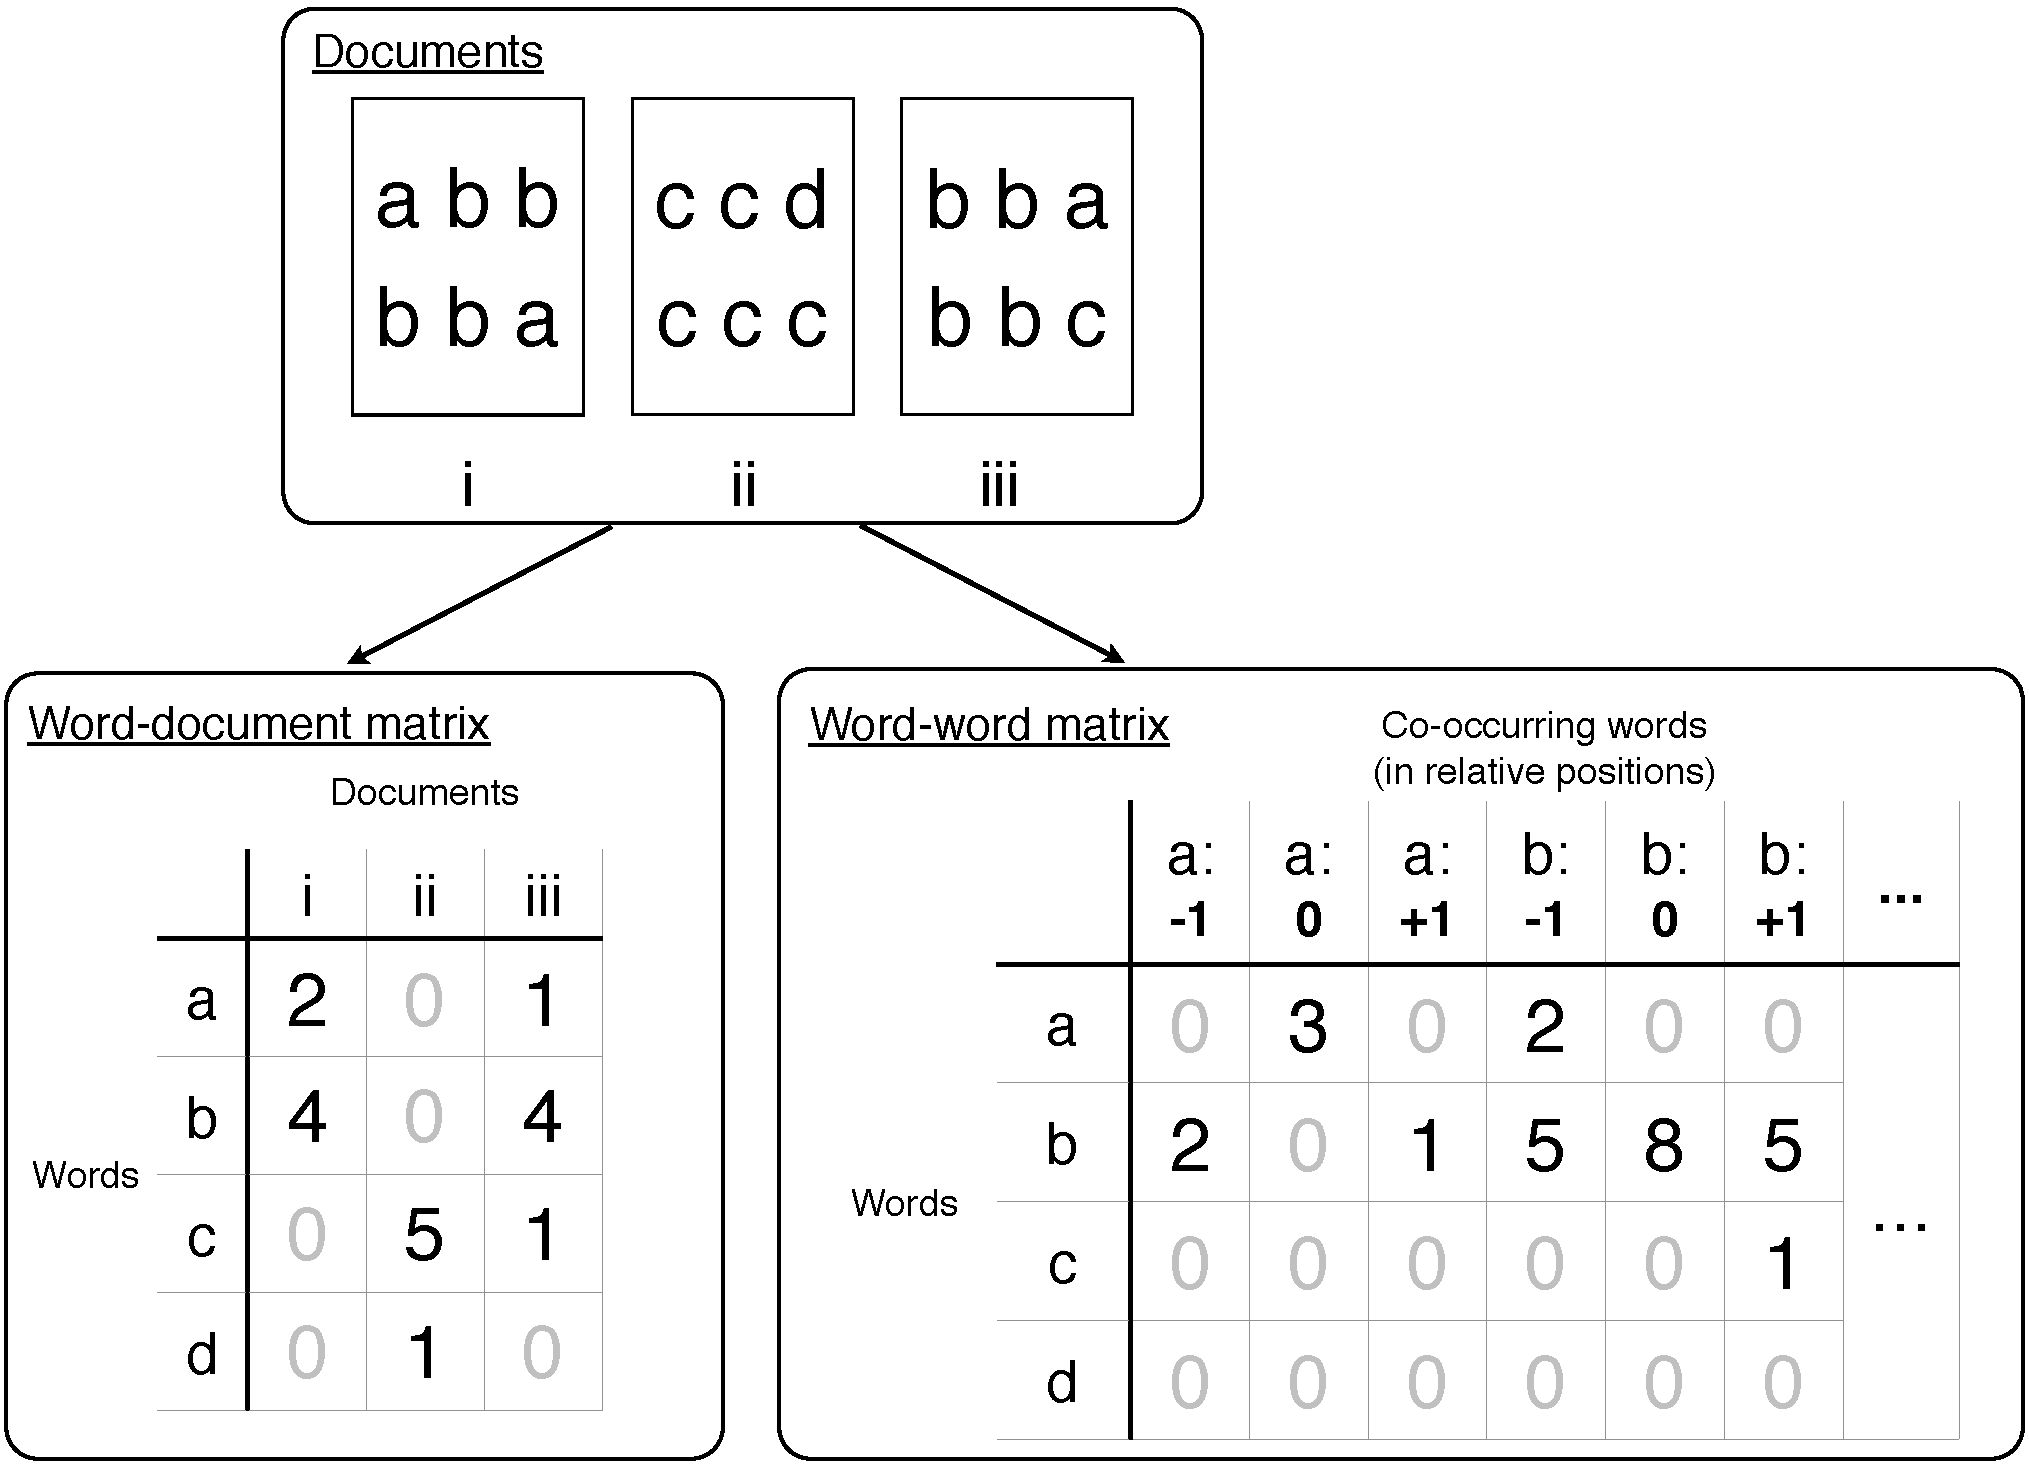
\includegraphics[width=0.9\linewidth]{matrices}
  \end{center}
  \caption{Word-document and word-word matrices. Word-document matrices measure how often words occur in particular documents. Word-word matrices measure how often pairs of words occur in certain relative positions.}
  \label{matrices}
\end{figure}

While such matrices can be interpreted as representing documents in terms of their constituent words, they can also be interpreted as representing words in terms of their patterns of use across documents, or, a proxy for the linguistic contexts that a word participates in. Put another way, such a matrix can be thought of either as a model of document meaning (i.e., a document's meaning is its column in this matrix) or, more importantly, for our purposes, a model of word meaning (i.e., a word's meaning is its row in this matrix). Note, however, that this word-document approach represents documents as ``bags'' of words---information about the relative position of words is discarded. The word-word approach retains this information \citep{church1990, schutze1992}. The word-word matrix has words as both rows and columns; a row might represent the meaning of word A and the count in a particular column might indicate frequency that word A occurred 2 words before word X (Figure \ref{matrices}).

Both word-document and word-word models are capable of learning semantic properties of words. In one influential model, \citet{landauer1997} developed a model called Latent Semantic Analysis (LSA), which builds a word-document matrix from a corpus, applies a dimensionality reduction technique (singular value decomposition), and computes the similarity between words using a cosine measure. After training on a corpus of encyclopedia articles, LSA closely matched the performance of non-native English speakers on a synonym test. In another model, \citet{redington1998} developed a model that performs hierarchical clustering on a word-word matrix. This model was able to learn syntactic (as opposed to semantic) categories like noun, verb, and adjective. An interesting feature of the learned clusters is that they often had semantic organization. For example, in the cluster of adjectives, the color words and number words formed separate clusters (p448). The success of early computational models led to a proliferation of models that learn from co-occurrence information (see \citealp{riordan2010} for an overview and comparison of state-of-the-art models). The computational evidence is quite strong: Statistical patterns of co-occurrence can, in principle, be used to learn \emph{inter alia} some aspects of word meaning.

There are computational proofs of concept, but there is little \emph{direct} evidence that humans use co-occurrence information to learn meaning. However, one influential case study offers some indirect evidence. \citet{shepard1992} presented congenitally blind, color-blind, and normally sighted participants with pairs of color words and asked them to make similarity ratings. As might be predicted, the ratings of blind participants did not correlate highly with normally sighted individuals. However, their ratings did appear to preserve the local similarity relationships---violet was rated most similar to purple, teal to green, and so forth. How might congenitally blind individuals have learned anything about color relationships? One possibility, raised by Shepard and Cooper, is that the blind may have extracted these relationships from their linguistic input. More recent work by \citet{bedny2012} has shown similar results with knowledge of visual verbs.

These demonstrations in the blind, while suggestive, are only indirect evidence of contextual co-occurrence learning. Researchers studying learning of syntactic categories (as opposed to word meanings) have employed methods that can in principle provide stronger evidence. These studies expose learners to artificial languages with certain co-occurrence regularities and measure whether learners form categories on the basis of these regularities. In the next section, we discuss results of studies that have examined a kind of co-occurrence structure, known as the MNPQ language.

\subsection{A puzzle: the MNPQ language}

The MNPQ language contains four categories of words, M (which includes $m_1$, $m_2$, and $m_3$), N ($n_1$, $n_2$, $n_3$), P ($p_1$, $p_2$, $p_3$), and Q ($q_1$, $q_2$, $q_3$). Participants hear two types of training sentences: MN and PQ. Thus, sentences like $m_1 n_3$ are grammatical while sentences like $m_1 q_3$ are illegal. Early investigations \citep{braine1966, smith1966} found that participants tend to endorse novel grammatical sentences as familiar. However, participants also endorse ungrammatical MQ and PN sentences, suggesting that they learn position regularities (that M/P come first and N/Q come second) but not co-occurrence regularities (that M co-occurs with N but not Q and that P occurs with Q but not N). This failure to learn categories on the basis of pure co-occurrence has been reliably observed in a number of studies \citep{braine1987, brooks1993, frigo1998, kempe2001, gerken2005, lany2010, frank2011}. However, \citet[Experiment 5]{reeder2009} report successful learning of a related language, (Q)AXB(R). In this language, there are optional Q and R categories that serve to deconfound co-occurrence regularities from positional regularities (i.e., in MNPQ, Ms and Ps are always sentence-initial and Ns and Qs are always sentence-final). However, it is difficult to directly compare (Q)AXB(R) and MNPQ results, due to the presence of an additional X category in the former; reconciling results from these two languages is a topic for future work. Nevertheless, the MNPQ failures are puzzling, given that computational models suggest that contextual co-occurrence learning is a powerful mechanism.

Many of same these studies have also demonstrated that MNPQ learning is possible, however, when co-occurrence information is partially or completely correlated with another cue. For example, \citet{braine1987} found that successful MNPQ learning results when co-occurrence information is partially correlated with natural gender. In this experiment, participants acquired an artificial language by learning to name pictures of referents. In the experimental condition, all pictures of men were labeled by Ms (though not all Ms referred to men) and all pictures of women were labeled by P words (though not all Ps referred to women). Learning of the co-occurrence regularities was significantly higher in the experimental condition than in a control condition where natural gender was not correlated with M/P membership. Though Braine's experiment combined co-occurrence cues with natural gender, he suggested that phonological cues might better serve real-world language learners. For instance, Spanish and Italian speakers might learn grammatical gender categories by taking advantage of the fact that feminine nouns often end with \emph{-a}, while masculine nouns often end with \emph{-o}. More generally, demonstrations that co-occurrence information can be useful in concert with other information sources have encouraged researchers to study how disparate sources might be integrated to facilitate learning (e.g., \citealp{monaghan2005, johns2012}).

Nearly all of this empirical work has interpreted the results of human experiments with reference to learning grammatical category, rather than word meaning. To our knowledge, only one study has examined word meaning. Recently, \citet{lany2010} investigated Braine's proposal of correlating co-occurrence and phonological cues in a study of meaning acquisition. They found that 22-month old infants successfully learned MNPQ when co-occurrence was aligned with the number of syllables in a word (in particular, when N words were disyllabic and Q words were monosyllabic) but \emph{not} when the number of syllables was not predictive of N/Q membership. This suggests that contextual co-occurrence may play a common role in acquisition of grammatical category and word meaning, at least for the MNPQ language. 

In our current work, we add to the literature on learning word meaning through contextual co-occurrence by exploring a new information source: semantic coherence. To date, all studies have used the artificial language learning paradigm. Thus, at the beginning of the experiments, learners did not know the meanings of any of the words. Real learners, by contrast, typically know the meanings of some (if not most) words they hear and such words tend to relate to a single topic of discourse. Put another way, the language that real learners encounter tends to have semantic coherence; some words are known and adhere to some semantic organization. We ask: does semantic coherence facilitate contextual co-occurrence learning?

To explore this possibility, we presented participants with an MNPQ language where sentences took the form ``M and N'' or ``P and Q''. Note that used an explicit English conjunction between the two words, which imbued sentences with semantic content (i.e., our stimuli were not merely a syntactic ordering). We hypothesized that a sufficient level of semantic coherence (specifically, a taxonomic coherence where Ms are animals and Ps were vehicles) would yield successful contextual co-occurrence learning for N and Q words . For instance, hearing the four sentences:
\begin{enumerate}
\item dog and dax
\item dog and ziv
\item car and wug
\item car and pif
\end{enumerate} might allow learners to infer that daxes and zivs belong to the same category, as both words co-occur with ``dog'', and that wugs and pifs belong to the same category, as both words co-occur with ``car''.

In Experiment 1, we tested whether semantic coherence facilitated contextual co-occurrence learning. In Experiment 2, we compared semantic coherence to phonological coherence. In Experiment 3, we compared semantic coherence to a semantic baseline that used known words that did not adhere to any obvious semantic organization.

\section{Experiment 1: Semantic Coherence}

In all the experiments reported in this paper, we presented participants with auditory sentences from an MNPQ language. In different conditions, we varied properties of the Ms (which co-occur with Ns) and Ps (which co-occur with Qs). We will call the Ms and Ps \emph{context words}. We measured learning for the Ns and Qs, which we will call the \emph{target words}.

In Experiment 1, we parametrically varied two independent properties of the context words. First, we manipulated semantic coherence---the fraction of M/P words obeying a taxonomic organization (M = animal words, P = vehicle words). Second, as one hallmark of statistical learning is sensitivity to the amount of evidence observed, we manipulated the amount of exposure to the language, in order to measure the efficiency of learning with respect to exposure amount. After participants were exposed to the language, we tested them on three measures of MNPQ learning---sentence memory, similarity rating, and a referent assignment task.

\subsection{Method}

\subsubsection{Participants}
678 Amazon Mechanical Turk (MTurk) workers. Using MTurk's worker qualifications, we limited participaton to workers located in the United States and with a previous HIT approval rate greater than or equal to 90\%. We chose MTurk workers as our participants because the number of experimental conditions required a large number of participants. Work by \citet{buhrmester2010} and \citet{crump2013} suggests that MTurk is a valid platform for web-based learning experiments.

\subsubsection{Materials}
Sentences took the form ``M and N'' or ``P and Q'' (Figure \ref{mnpq-table}). Note that sentences literally included the word ``and'' in the middle. We generated the actual lexical items randomly for each participant. Ns and Qs were always novel nonsense words and were drawn without replacement from the set \{moke, thite, jiv, pif, dex, wug\}. Ms and Ps could be either novel or familiar. Novel Ms were drawn from \{feeb, bim, lup\} and novel Ps were drawn from \{zabe, vap, chuv\}. Familiar Ms and Ps obeyed a taxonomic organization---familiar Ms were drawn from \{hamster, cat, dog\} and familiar Ps were drawn from \{car, bus, truck\}.

To create the audio files, we input the sentences as ``X. and. Y.'' (e.g., ``car. and. chuv.'', including periods) into an American English text-to-speech engine using a female voice.\footnote{\label{tts}We programatically submitted all of our sentences to the text-to-speech web service that powers Google Translate. During our investigation, the set of voices on the web service changed, which required us to synthesize our stimuli using different software. See also Footnote \ref{change-of-stimuli}.} The periods between words introduced substantial pauses ranging in length from 150 to 300 ms; piloting revealed that without pauses, it was difficult for participants to distinguish the words. Sentences using only monosyllabic words were around 2 seconds long. Sentences using the sole disyllabic word, hamster, were around 3 seconds long.  The referent assignment task involved visual referents. For the context words, we used 128x128 pixel images of a cat, dog, hamster, car, bus, and truck. For the target words, we used 100x100 pixel images of a horse, rabbit, sheep, bear, goldfish, mouse, boat, van, train, motorcycle, plane, and bicycle.

\begin{figure}[t]
  \begin{center}
    \begin{tabular}{ p{0.3\linewidth} p{0.35\linewidth} p{0.35\linewidth} }
      %% HT the comment from Herbert on http://tex.stackexchange.com/a/58314
      \vspace{0pt}
      \begin{tabular}{ l l l }
        \multicolumn{3}{c}{Exposure sentences}\\
        \underline{$m_1$ $n_1$} & $m_1$ $n_2$ & $m_1$ $n_3$  \\
        $m_2$ $n_1$ & \underline{$m_2$ $n_2$} & $m_2$ $n_3$  \\
        $m_3$ $n_1$ & $m_3$ $n_2$ & \underline{$m_3$ $n_3$}  \\
        \underline{$p_1$ $q_1$} & $p_1$ $q_2$ & $p_1$ $q_3$ \\
        $p_2$ $q_1$ & \underline{$p_2$ $q_2$} & $p_2$ $q_3$ \\
        $p_3$ $q_1$ & $p_3$ $q_2$ & \underline{$p_3$ $q_3$} \\
      \end{tabular} 

      & 

      \vspace{0pt}
      \begin{tabular}{l l}
        \multicolumn{2}{c}{Memory items}\\
        Sentence type & Example\\
        \hline
        Familiar & $m_1$ $n_2$\\
        Withheld & $m_1$ $n_1$\\
        Category violation & $m_1$ $q_2$\\
        Pair violation & $m_1$ $m_1$\\
        \hline
      \end{tabular}

      &

      \vspace{0pt}
      \begin{tabular}{l l}
        \multicolumn{2}{c}{Similarity items}\\
        Pair type & Example\\
        \hline
        Within-category & $n_1$, $n_2$\\
        Cross-category & $n_1$, $q_1$\\
        \hline
      \end{tabular}
    \end{tabular}
    \caption{The MNPQ language and test items for memory and similarity. Underlined sentences were withheld from exposure.}
    \label{mnpq-table}
  \end{center}
\end{figure}


\subsubsection{Design and Procedure}

We parametrically varied coherence. The language for a participant contained either 0/3, 1/3, 2/3, or 3/3 familiar M and P words each. We also varied the amount of exposure to the language---participants heard either 56, 126, 196, or 392 sentences. Before starting the experiment, we asked participants to turn on their speakers and click a button, which played a spoken English word (``airplane''). Participants were required to type the word correctly to continue. The experiment had four phases: exposure, similarity, memory, and referent assignment. Below, we detail these phases.

\paragraph{Exposure}
Participants listened to sentences from the language. We withheld six sentences from exposure (Figure \ref{mnpq-table}), yielding 14 unique sentences in the exposure set. Each sentence was heard either 4, 9, 14, or 28 times, giving 56, 126, 196, or 392 total trials. We presented the sentences in random order subject to the constraint that there were no repeated words between consecutive trials (pilot testing suggested that repeated words between trials substantially afforded learning). To encourage compliance, participants had to click a button to hear each sentence.

\paragraph{Similarity}
For each pair of words in the union of N and Q, we asked participants to rate on a 5 point scale how similar they believed the two words to be in meaning. This resulted in within-category judgments (e.g., $n_1$ vs. $n_2$) and cross-category judgments (e.g., $n_1$ vs. $q_1$). We presented the pairs in a fixed pseudorandom order containing no repeated words between consecutive trials. Though exposure was entirely auditory, for convenience, we presented these similarity questions as text (e.g., ``How similar are \textbf{pif} 
\includegraphics[width=0.3cm]{play.png} and \textbf{thite} 
\includegraphics[width=0.3cm]{play.png} ?''); to facilitate mapping between visual and spoken word forms, the speaker button next to each word played the spoken word when clicked. In two catch trials, participants were asked to press the response button corresponding to the solution of a simple arithmetic problem. If participants learned the MN and PQ co-occurrence relationships \emph{and} used these relationships as a basis for lexical categorization, then we expected that within-category pairs of words would be judged to be more similar than cross-category pairs.

\begin{figure}[t]
  \begin{center}
    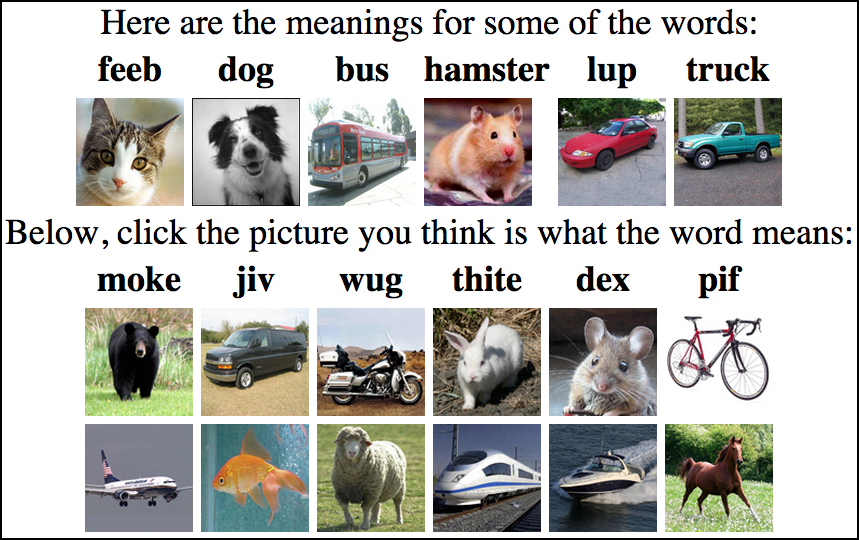
\includegraphics[width=8.5cm]{meaning-html-cropped.png}
    \caption{A screenshot of the referent assignment task.}
    \label{meaning-task}
  \end{center}
\end{figure}

\paragraph{Memory}
Participants listened to sentences and judged on a 5 point scale how confident they were that they had previously heard the sentence during exposure. We tested four types of sentences:

\begin{itemize}
\item \emph{Familiar} sentences heard during exposure.
\item \emph{Withheld} sentences not heard during exposure but
conforming to the MNPQ structure.
\item \emph{Cross-category} sentences of the form MQ and PN.
\item \emph{Pair violation} sentences of the form MM, NN, PP, and
QQ.
\end{itemize}

Sentences were presented in random order such that there were no repeated words between consecutive trials. In two catch trials,\footnote{In initial data collection, we did not include catch trials.  Let [A/3;B] denote the experimental condition with A/3 coherence and B exposures (e.g., [2/3;196] refers to the 2/3 coherence level with 196 exposures). In [0/3;196], 18 out of 40 participants did not receive catch trials. In [3/3;56], 30 out of 43 participants did not receive catch trials. In [3/3;126], 30 out of 40 participants did not receive catch trials. In [3/3;196], 30 out of 40 participants did not receive catch trials.} instead of a sentence from the MNPQ language, we played a non-repeatable audio instruction to press a specific response button.  If participants learned the MN and PQ co-occurrence relationships, then we expected that they would rate novel grammatical sentences as more familiar than the cross-category sentences.

\paragraph{Referent assignment}
We provided participants with meanings for all of the Ms and Ps and asked them to choose meanings for the Ns and Qs (Figure \ref{meaning-task}). At the top of the screen, we displayed the Ms and Ps in random order and we provided meanings by displaying a single image underneath each word. The M and P referents were either animals (cat, dog, hamster) or vehicles (car, bus, truck); either Ms were animals and Ps were vehicles, or vice versa. Recall that some conditions contained \emph{familiar} M and P words; in these cases, we paired the known words with the obvious referents (e.g., ``dog'' was always paired with an image of a dog). Below the M and P words and their meanings, we displayed a row containing the N and Q words. Under each word, we displayed a two-alternative referent choice between an animal (the ``correct'' choice for N words) and vehicle words (the ``correct'' choice for Q words); participants made a choice by clicking on one of the two pictures. If participants learned the MN and PQ co-occurrence relationships \emph{and} used them to form nascent lexical categories \emph{and} used these lexical categories as a basis for inferences about word meaning, then we expected that referent assignment scores would reflect a tendency to choose on the basis of the taxonomic categories of the co-occurring words (e.g., Ns should be animals because they co-occur with Ms, which are known to be animals).

% To summarize, we devised three measures of learning: (1) memory for sentences, (2) similarity between target words, and (3) inductive bias in referent assignment.

\subsection{Results and Discussion}
We excluded the 55 participants who did not correctly answer all of the catch trials. Results are shown in Figure \ref{expt1-results}. For each dependent measure---memory, similarity, and meaning---we defined a within-participant score representing the sensitivity to the co-occurrence regularities in the language. Memory score was the difference in mean ratings between novel withheld sentences (e.g., $m_1$--$n_1$) and novel category violation sentences (e.g., $m_1$--$q_1$). Similarity score was the difference between mean ratings of within-category (e.g., $N$--$N$) and cross-category (e.g $N$--$Q$) ratings. Referent assignment score was the total number of correct choices in the referent assignment task. All scores were normalized to the interval [-1, 1].

\subsubsection{Analysis approach}
Using linear models, we analyzed two aspects of the data. First, we were interested in main effects of coherence on score (i.e., the Condition coefficients in Table \ref{expt1-regressions}). Second, we were interested in the relationship between amount of exposure and score. Accordingly, we looked for exposure $\times$ coherence interactions. A significant interaction (e.g., the E $\times$ C coefficients in Table \ref{expt1-regressions}) would indicate a difference in how \emph{efficiently} the statistical learning process makes use of evidence at different coherence levels. For all scores, we coded coherence as a categorical variable and analyzed the data using a regression which modeled the mean score in a participant group (e.g., 3/3-56) as an interactive function of the number of exposures (e.g., 56) times the condition (e.g., full coherence). In other words, our regression equation was score $\sim$ exposures $\times$ condition.

To examine the differences between the different coherence levels, we used Helmert contrasts analyzing (i) the difference between the 1/3 and 0/3 conditions, (ii) the difference between the 2/3 condition and the 0/3 and 1/3 conditions combined, and (iii) the difference between the 3/3 condition and the 0/3, 1/3, and 2/3 conditions combined. Results of these analyses are shown in Table \ref{expt1-regressions}.

Before detailing the results for each measure, we will first state the two broad patterns of results. First, learning was highest in 3/3 condition. Second, we found the strongest evidence of statistical efficiency (i.e., sensitivity to the amount of exposure) in the 3/3 condition.

\begin{figure}[t]
  \begin{center}
    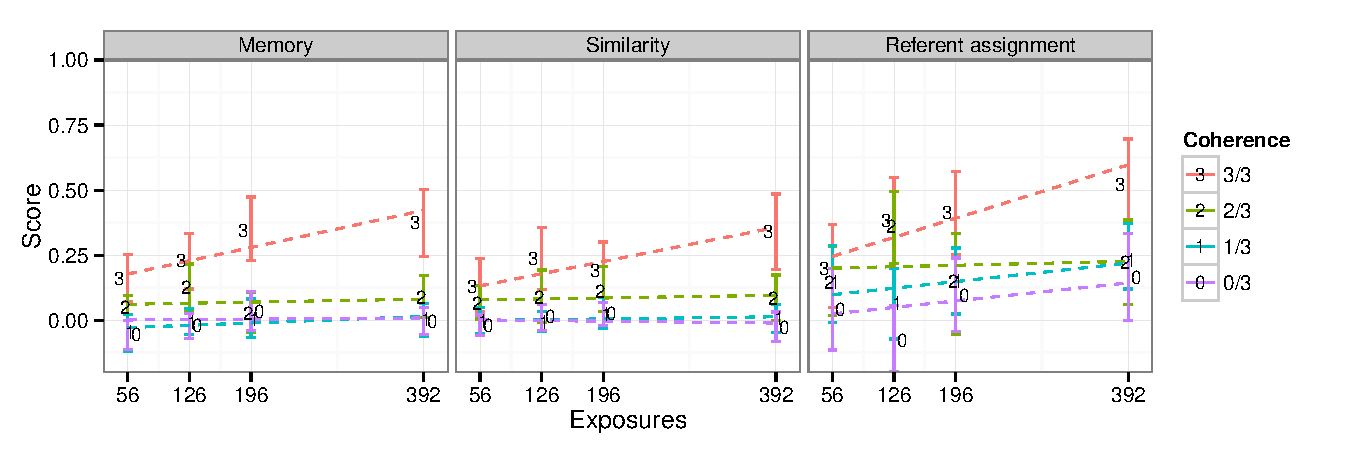
\includegraphics[width=1.0\linewidth]{x1}
    \caption{Experiment 1 results. Each plot shows data for one
measure (memory, similarity, meaning) in Experiment 1. Points show
condition means, error bars show 95\% CIs, and dashed lines show the
best-fitting linear regression.}
    \label{expt1-results}
  \end{center}
\end{figure}

\newcommand{\ww}{\color{white}{*}} \newcommand\T{\rule{0pt}{2.1ex}}

\begin{table}[ht]
  \caption{Regression model for Experiment 1. For readability, exposure values were divided by 1000.}
  \label{expt1-regressions} 
  \begin{center}
  \footnotesize{
    \begin{tabular}{l r r r r}
      \hline
      Regressor & $\beta$ & Std Error & $t$ & $p$ \\ \hline
      \multicolumn{5}{c}{\T Memory \T}\\
      Intercept &  0.0359 &  0.018 &  1.91 & 0.056\ww\\
      Condition: 1/3 -- (0/3) & -0.0005 &  0.027 & -0.01 & 0.984\ww\\
      Condition: 2/3 -- (0/3,1/3) &  0.0309 &  0.014 &  2.09 & <0.05*\\
      Condition: 3/3 -- (0/3,1/3,2/3) &  0.0396 &  0.010 &  3.65 & <0.001*\\
      Exposures &  0.2346 &  0.083 &  2.81 & <0.005*\\
      E $\times$ C: 1/3 -- (0/3) &  0.0033 &  0.120 &  0.02 & 0.977\ww\\
      E $\times$ C: 2/3 -- (0/3,1/3) & -0.0215 &  0.065 & -0.32 & 0.743\ww\\
      E $\times$ C: 3/3 -- (0/3,1/3,2/3) &  0.1326 &  0.048 &  2.73 & <0.01* \\
      \hline

      \multicolumn{5}{c}{\T Similarity \T}\\
      Intercept &  0.0501 &  0.018 &  2.64 & <0.01*\\
      Condition: 1/3 -- (0/3) & -0.0070 &  0.027 & -0.25 & 0.798\ww\\
      Condition: 2/3 -- (0/3,1/3) &  0.0237 &  0.014 &  1.59 & 0.112\ww\\
      Condition: 3/3 -- (0/3,1/3,2/3) &  0.0224 &  0.010 &  2.04 & <0.05*\\
      Exposures &  0.1487 &  0.084 &  1.77 & 0.077\ww\\
      E $\times$ C: 1/3 -- (0/3) &  0.0514 &  0.121 &  0.42 & 0.671\ww\\
      E $\times$ C: 2/3 -- (0/3,1/3) &  0.0208 &  0.066 &  0.31 & 0.754\ww\\
      E $\times$ C: 3/3 -- (0/3,1/3,2/3) &  0.1373 &  0.048 &  2.80 & <0.01* \\
      \hline

      \multicolumn{5}{c}{\T Referent assignment \T}\\
      Intercept &  0.1087 &  0.036 &  3.01 & <0.005*\\
      Condition: 1/3 -- (0/3) &  0.0664 &  0.052 &  1.26 & 0.208\ww\\
      Condition: 2/3 -- (0/3,1/3) &  0.0616 &  0.028 &  2.17 & <0.05*\\
      Condition: 3/3 -- (0/3,1/3,2/3) &  0.0359 &  0.020 &  1.72 & 0.084\ww\\
      Exposures &  0.4577 &  0.159 &  2.86 & <0.005*\\
      E $\times$ C: 1/3 -- (0/3) & -0.0919 &  0.230 & -0.39 & 0.690\ww\\
      E $\times$ C: 2/3 -- (0/3,1/3) & -0.1257 &  0.126 & -0.99 & 0.319\ww\\
      E $\times$ C: 3/3 -- (0/3,1/3,2/3) &  0.1292 &  0.093 &  1.38 & 0.167\ww \\
      \hline
    \end{tabular}
  }
  \end{center}
\end{table}

\subsubsection{Task results}

We report performance on each of the three tasks separately

\paragraph{Memory} There was a significant main effect of exposure, with greater exposure resulted in better memory scores. There was also a significant main effect of condition; 2/3 scores were significantly higher than scores from the 0/3 and 1/3 conditions combined and 3/3 scores were significantly higher than scores from the rest of the conditions combined. Because 2/3 and 3/3 scores both outperformed all the respective lower levels of coherence, we also computed this model using coherence as a continuous variable; the continuous coherence regressor significantly predicted increases in score, $\beta = 0.06$, $t(619) = 3.86$, $p < 0.0005$, suggesting that \emph{parametrically} increasing coherence results in \emph{parametric} increases in memory score.

% condition.num 6.730e-02 1.743e-02 3.862 0.000124 ***

Additionally, there was a significant exposure $\times$ condition interaction; the effect of exposures on score was significantly higher in 3/3 than in the other conditions combined, suggesting greater efficiency of statistical learning in 3/3. Thus, more semantically coherent linguistic input (1) bolstered memory for the $MN$ and $PQ$ co-occurrence regularities and (2) increased the efficiency of the statistical learning process responsible for learning those regularities, at least in the 3/3 condition.

\paragraph{Similarity} There was a significant main effect of condition: 3/3 scores were significantly higher than in the other conditions combined. Additionally, there was a significant exposure $\times$ condition interaction; the effect of exposures on score was significantly higher in 3/3 than in the other conditions combined. Thus, more coherent linguistic input (1) increased the distinction between within-category and cross-category pairs of words and (2) increased the efficiency of the statistical learning process involved in making such distinctions, at least in the 3/3 condition.

\paragraph{Referent assignment}

There were significant main effects of exposure and condition. 2/3 scores were significantly higher than 0/3 and 1/3 scores combined. 3/3 scores were marginally higher than the rest of the scores combined, $\beta = 0.03, t(615) = 1.72, p = 0.08$, possibly because 3/3 coherence and 2/3 coherence may confer comparable advantages on this task. We also computed this model using coherence as a continuous variable; the continuous coherence regressor significantly predicted increases in score, $\beta = 0.09$, $t(619) = 2.87$, $p < 0.005$, suggesting that \emph{parametrically} increasing coherence results in \emph{parametric} increases in referent assignment score. None of the interaction terms reached significance, indicating that the amount of exposure to the language and greater coherence independently increased the ability to assign $N$ and $Q$ words to the correct referents.

% parametric increase stuff: condition.num 9.434e-02 3.285e-02 2.872 0.00422 **

\subsubsection{Integrative results} Why does semantic coherence facilitate MNPQ learning? \citet{frank2011} have shown that MNPQ learning can be bolstered by easing working memory demands. Additionally, there is evidence that novel words tax the memory system more, as they are encoded in terms of smaller phonological units \citep{treiman1988}. So it is possible that semantic coherence improved MNPQ learning by reducing memory demands.

We tested for this possibility in our data using mediation analyses. In particular, we tested whether memory scores mediated the effect of coherence on either (1) similarity scores or (2) referent assignment scores. In both cases, we found partial mediation. After controlling for memory, the regression coefficient relating coherence and similarity decreased significantly from $0.07$ to $0.03$, Sobel $z$ = 7.80, $p < 0.005$; this reduced value was significantly greater than zero, $t(620) = 3.50, p < 0.001$, indicating partial mediation. After controlling for memory, the regression coefficient relating coherence and referent assignment score decreased significantly from $0.10$ to $0.05$, Sobel $z$ = 5.33, $p < 0.005$; this reduced value was significantly greater than zero, $t(616) = 3.15, p < 0.005$, again indicating partial mediation. Thus, improved memory can explain some, but not all, of the increase in similarity and referent assignment scores due to semantic coherence.

\subsubsection{Summary}

In Experiment 1, we found that semantic coherence (1) increased ability to distinguish novel grammatical sentences from sentences violating co-occurrence regularities in the memory task, (2) sharpened sensitivity to lexical category boundaries based on the co-occurrence regularities in the similarity task, and (3) increased inductive bias in associating words with objects in the referent assignment task. Using mediation analysis, we found that evidence that semantic coherence boosts learning in part because it eases memory demands.

Semantic coherence has two components: meaning and coherence. How does the effect of semantic coherence depend on each? In Experiments 2 and 3, we test for the effect of meaning and coherence respectively. In Experiment 2, we remove meaning by exposing learners to languages with phonological, as opposed to semantic, coherence. In Experiment 3, we remove coherence by exposing learners to languages with context words that are familiar but do not adhere to any obvious semantic organization.

\section{Experiment 2: Phonological coherence}

In Experiment 2, we investigated whether learners could learn the language used in  Experiment 1 when the context words (Ms and Ps) exhibited phonological, rather than semantic, coherence. We tested three types of coherence: onset, rime, and syllable count.

\subsection{Method}
\subsubsection{Participants} 
530 MTurk workers, recruited as in Experiment 1, participated in the study.

\subsubsection{Materials}
The three types of phonological coherence\footnote{\label{change-of-stimuli} The stimuli for the rime and syllable count conditions differ from those in the rest of our conditions. For the rest of the conditions, we used a text-to-speech web service provided by Google to generate the audio stimuli (see Footnote \ref{tts}) for the bulk of the conditions. However, the available voices on this service changed during our experiment. Thus, we generated new stimuli for the rime and syllable count conditions using commercially available software, NaturalReader 10. To ensure that the old and new stimuli were comparable, we performed a partial replication of Experiment 1 using the new synthesis engine; the difference old and new stimuli did not appear to make a substantial difference. See Appendix \ref{old-vs-new} for comparisons.} were:

\begin{itemize}
\item \emph{Onset}. Ms all started with one consonant cluster (pladge, plaaf, plab) and Ps all started with another (zof, zawd, zawsh).
\item \emph{Rime}. Ms all ended with one vowel (calo, pawmo, marfo) and Ps all ended with another (zaygee, kaisee, tetchee).
\item \emph{Syllable count}. Ms were disyllabic (coomo, fengle, kaisee) and Ps were monosyllabic (gope, jic, skeege).
\end{itemize}

\subsubsection{Design and Procedure}
The method was identical to that of Experiment 1.

\subsection{Results and Discussion}

\begin{figure}[t]
  \begin{center}
    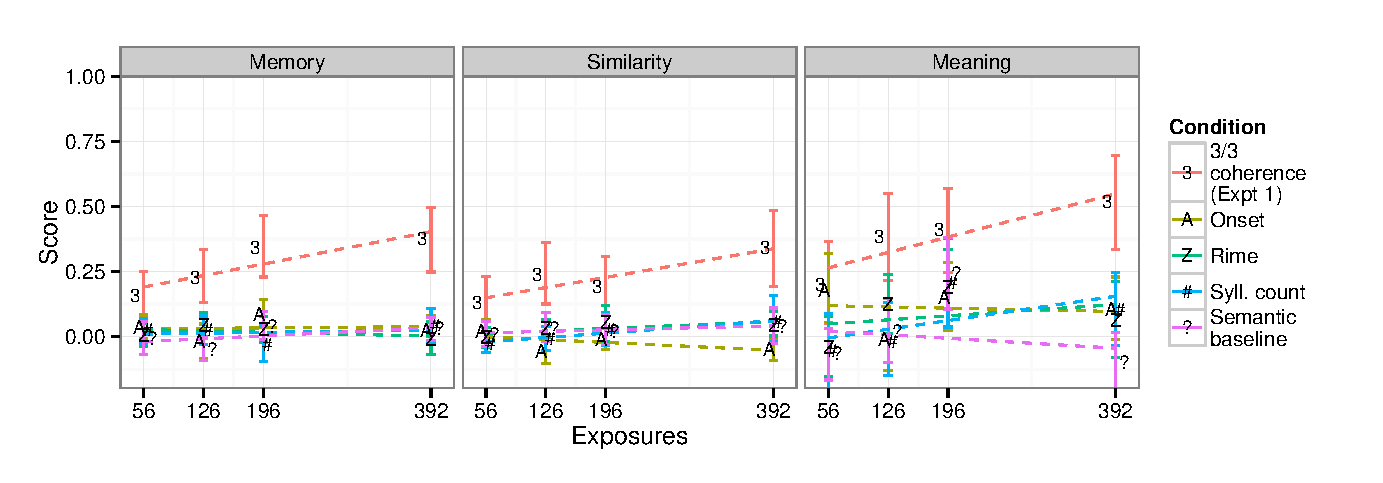
\includegraphics[width=1.0\linewidth]{x23}
    \caption{Experiments 2 and 3 results. Each plot shows data for one
      measure (memory, similarity, meaning). Points show condition means,
      error bars show 95\% CIs, and dashed lines show the best-fitting
      linear trend. For comparison, we also include the 3/3 coherence
      condition from Experiment 1.}
    \label{expt23-results}
  \end{center}
\end{figure}

\begin{table}[t]
  \caption{Regression model for Experiments 2 and 3. For readability, exposure values were divided by 1000.}
  \label{expt23-regression}
  \begin{center} 
    \scriptsize{
      \begin{tabular}{l r r r r}
        \hline
        Predictor & $\beta$ & Std Error & $t$ & $p$ \\ \hline
        \multicolumn{5}{c}{\T Memory \T}\\
        Intercept & -0.0341 &  0.027 & -1.24 & 0.215\ww\\
        Condition: Onset -- 0/3 &  0.0626 &  0.038 &  1.64 & 0.100\ww\\
        Condition: Rime -- 0/3 &  0.0652 &  0.035 &  1.82 & 0.068\ww\\
        Condition: Syllable count -- 0/3 &  0.0410 &  0.038 &  1.06 & 0.287\ww\\
        Condition: Semantic incoherent -- 0/3 &  0.0055 &  0.038 &  0.14 & 0.883\ww\\
        Exposures &  0.1201 &  0.119 &  1.00 & 0.316\ww\\
        E $\times$ C: Onset -- 0/3 & -0.0948 &  0.170 & -0.55 & 0.577\ww\\
        E $\times$ C: Rime -- 0/3 & -0.1950 &  0.161 & -1.20 & 0.228\ww\\
        E $\times$ C: Syllable count -- 0/3 & -0.0735 &  0.167 & -0.43 & 0.660\ww\\
        E $\times$ C: Semantic incoherent -- 0/3 &  0.0388 &  0.162 &  0.23 & 0.811\ww \\
        \hline

        \multicolumn{5}{c}{\T Similarity \T}\\
        Intercept &  0.0110 &  0.025 &  0.43 & 0.662\ww\\
        Condition: Onset -- 0/3 & -0.0031 &  0.035 & -0.08 & 0.928\ww\\
        Condition: Rime -- 0/3 & -0.0064 &  0.033 & -0.19 & 0.846\ww\\
        Condition: Syllable count -- 0/3 & -0.0455 &  0.035 & -1.27 & 0.201\ww\\
        Condition: Semantic incoherent -- 0/3 & -0.0007 &  0.035 & -0.02 & 0.982\ww\\
        Exposures & -0.0607 &  0.110 & -0.54 & 0.582\ww\\
        E $\times$ C: Onset -- 0/3 & -0.0937 &  0.157 & -0.59 & 0.550\ww\\
        E $\times$ C: Rime -- 0/3 &  0.1951 &  0.149 &  1.30 & 0.191\ww\\
        E $\times$ C: Syllable count -- 0/3 &  0.3049 &  0.154 &  1.97 & <0.05*\\
        E $\times$ C: Semantic incoherent -- 0/3 &  0.1401 &  0.150 &  0.93 & 0.350\ww \\
        \hline

        \multicolumn{5}{c}{\T Referent assignment \T}\\
        Intercept & -0.0553 &  0.068 & -0.81 & 0.418\ww\\
        Condition: Onset -- 0/3 &  0.1776 &  0.094 &  1.88 & 0.060\ww\\
        Condition: Rime -- 0/3 &  0.0916 &  0.088 &  1.03 & 0.301\ww\\
        Condition: Syllable count -- 0/3 &  0.0234 &  0.095 &  0.24 & 0.806\ww\\
        Condition: Semantic incoherent -- 0/3 &  0.0868 &  0.094 &  0.91 & 0.359\ww\\
        Exposures &  0.5462 &  0.296 &  1.84 & 0.066\ww\\
        E $\times$ C: Onset -- 0/3 & -0.6122 &  0.421 & -1.45 & 0.146\ww\\
        E $\times$ C: Rime -- 0/3 & -0.3243 &  0.400 & -0.80 & 0.418\ww\\
        E $\times$ C: Syllable count -- 0/3 & -0.0692 &  0.414 & -0.16 & 0.867\ww\\
        E $\times$ C: Semantic incoherent -- 0/3 & -0.7403 &  0.402 & -1.83 & 0.066\ww \\
        \hline
      \end{tabular}
    }
  \end{center}
\end{table}

We discarded the 42 participants who did not pass all the catch trials. Results are graphed in Figure \ref{expt23-results}. Using a regression model with main effects of exposure and condition and an exposure $\times$ condition interaction, we compared each phonological condition with the 0/3 condition of Experiment 1 using a regression model (Table \ref{expt23-regression}).

\subsubsection{Memory}
There was no main effect of exposure. There was also no main effect of condition---none of the phonological condition scores were significantly different from 0/3 scores. None of the exposure by condition interaction terms were significant.

\subsubsection{Similarity}
Again, we found no main effect of exposure or condition. One interaction term was significant: there appeared to be greater efficiency of statistical learning in the syllable count condition than in the 0/3 condition.

\subsubsection{Referent assignment}
Again, we found no main effect of exposure or condition. None of the exposure by condition interaction terms were significant.

Across the three models, there were no significant predictors, save the one interaction term for syllable count versus 0/3 on the similarity measure, which can be plausibly attributed to chance. This suggests that phonological coherence was virtually indistinguishable from the 0/3 condition in terms of facilitating MNPQ learning. This indicates that mere phonological coherence is not what drives the effects of semantic coherence. In Experiment 3, we consider whether the mere presence of known words (semantic baseline) aids MNPQ learning.

\section{Experiment 3: Semantic baseline}

In Experiment 1, Ms and Ps were all familiar words obeying a taxonomic organization. In Experiment 3, we explored whether mere coherence is sufficient for facilitation of contextual co-occurrence learning, or whether the mere presence of known words is sufficient---that is, whether a semantically baseline language facilitates contextual co-occurrence learning. We might expect this baseline condition to facilitate learning due to lower memory demands---known words tax the memory system less, which might free learners to identify co-occurrence regularities.

\subsection{Methods}
\subsubsection{Participants}
162 MTurk workers, recruited as in Experiment 1.

\subsubsection{Materials}
In the semantic baseline language, the specific M and P words were drawn randomly for each participant from the pool \{\emph{shelf}, \emph{glove}, \emph{rain}, \emph{leash}, \emph{card}, \emph{ball}\}. In the referent assignment task, these known words were paired with images of the obvious referents (e.g., \emph{card} with a picture of a card).

\subsubsection{Design and procedure}
The method was identical to that of Experiment 1.

\subsection{Results and Discussion}
We discarded the 18 participants who did not pass all the catch trials. Results are graphed in Figure \ref{expt23-results}. See Table \ref{expt23-regression} for regression results.

\subsubsection{Memory}
Baseline scores were not significantly different from 0/3 scores and baseline efficiency was not significantly different from 0/3 efficiency.

\subsubsection{Similarity}
Baseline scores were not significantly different from 0/3 scores and baseline efficiency was not significantly different from 0/3 efficiency.

\subsubsection{Referent assignment}
Baseline scores were not significantly different from 0/3 scores and baseline efficiency was not significantly different from 0/3 efficiency.\\

Apparently, the baseline input appeared to have provided no benefit compared to the novel words of the 0/3 condition, suggesting that the presence of known words by itself does not aid MNPQ learning.

\section{General Discussion}

How people learn word meanings remains a central problem in cognitive science. In this paper, we have explored whether people might learn meaning from language itself, using patterns of co-occurrence as a clue towards word meaning. Previous work on contextual co-occurrence learning presented a paradox: while computational models suggest that contextual co-occurrence is a powerful source of information, human experiments show consistent failures without correlated information sources, such as natural gender \citep{braine1987} or phonological regularities \citep{frigo1998, monaghan2005, lany2010}. Learning experiments typically present participants with linguistic input that is entirely novel, whereas real learners generally know the meanings of some of the words. Thus, we investigated learning in settings where some words are familiar and have a semantic organization, a factor we call semantic coherence. Our experiments show that semantic coherence facilitates MNPQ learning. When a sufficient fraction of context words were familiar and obeyed a taxonomic organization, our participants successfully learned categories on the basis of contextual co-occurrence. Furthermore, data from the referent assignment task suggest that participants were willing to make inferences about word meaning for these categories.

In Experiment 1, we showed that semantic coherence facilitates MNPQ learning; 3/3 semantic coherence resulted in better memory for the co-occurrence structure of the language and sharper inductive bias in similarity and meaning judgments. Additionally, for the memory and similarity measures, we found evidence of greater statistical efficiency---using regression, we found that the 3/3 rate of learning was higher than the other conditions. In Experiments 2 and 3, we investigated whether the effect of semantic coherence was driven by either meaning or coherence alone. In Experiment 2, we kept coherence but removed meaning by testing languages with phonological coherence. These languages did not confer any learning benefits, indicating that coherence alone does not drive the effect of semantic coherence. In Experiment 3, we kept meaning but removed coherence by testing a baseline language with known words but no obvious semantic organization. This language did not confer any learning benefits, indicating that meaning alone does not drive the effect of semantic coherence. It appears that the interaction of both meaning and coherence drives the effect; when we separately removed meaning (as in the phonological conditions) and coherence (as in the semantic baseline condition), learners failed to learn co-occurrence regularities in the language.

That phonological coherence did not facilitate learning is somewhat at odds with previous work \citep{frigo1998, monaghan2005, lany2010}. However, whereas previous work has applied phonological regularities to the \emph{target} words (i.e., the words that experimenters measure learning for), we applied the regularities to the \emph{context} words (i.e., the words that co-occurred with the target words) in order to permit comparison with our semantic coherence conditions. Our operationalization of phonological coherence therefore differs from previous experiments. In our experiments, target words had \emph{second-order} phonological coherence; the target categories themselves did not have phonological regularity but they reliably co-occured with context categories that did. By contrast, in previous experiments \citet{lany2010}, target categories had \emph{first-order} coherence: the target categories themselves had phonological regularities (and context categories did not). Both types of coherence have theoretical motivations. \citet{braine1987} observed that first-order coherence occurs in languages like Spanish and Italian, where gender is marked on the noun (e.g., words that end in \emph{-o} tend to be masculine). We note that second-order coherence occurs in languages like Russian, which mark a noun's gender on the verb. Thus, contextual co-occurrence learning may be sensitive to differences in the kind of phonological coherence.

% As we mentioned in the introduction, most empirical work on MNPQ and contextual co-occurrence learning has focused on acquisition of \emph{syntactic categories}. However, the earliest inspiration for this research posited a link between co-occurrence and \emph{meaning}. Researchers (e.g., Lany \& Saffran, 2010) are starting to direct attention back towards meaning. Our work is in this vein. Because we found an effect of semantic coherence on the referent selection task, our results indicate that semantic coherence facilitates acquisition of meaning. Of course, we also find effects of semantic coherence in our memory and similarity tasks, which are arguably less semantic in nature. Based on this pattern of results, we believe that contextual co-occurrence learning, at its heart, acquires unlabeled categories. These unlabeled categories, in turn, can be used in the formation of explicitly syntactic or semantic categories. This suggests a degree of commonality between syntactic and semantic categories, which we believe is consistent with computational results on syntax. For example, Redington, Chater, and Finch (1998) developed a contextual co-occurrence learning model for syntactic category; many of the model's acquired clusters exhibited semantic organization (e.g., separate clusters of color and number words).

%%% commented out because this might contradict the proposed discourse-topic-inference method. 
%%% also, people can't actually do unsupervised MNPQ learning, so maybe it's NOT about unlabeled categories 

Our experiments highlight a limitation of artificial language learning paradigms. Researchers using entirely artificial languages may be severely limiting the power of contextual co-occurrence learning, which our experiments show to be greatly enhanced by the presence of known words that adhere to some semantic organization. In our analyses, memory was a significant (albeit partial) mediator of the effect of semantic coherence on similarity and referent assignment scores. Thus, artificial languages may place too high a memory burden on learners \citet{frank2011}. To better match experimental settings with conditions that real language learners find themselves in, we argue for more research using ``semi-artificial'' languages. Alternatively, it may be possible to mimic semantic organization in entirely artificial languages by seeding sentences with nonce topics (e.g., ``the sentence you are about to hear is about \emph{chylu}'').

Our empirical results can serve as a useful testbed for computational models. Surprisingly, work on contextual co-occurrence learning of semantics (and syntax) has generally been either empirical or computational: the two are rarely combined (cf. \citealp{qian2012}).  In computational work, researchers typically train models on large corpora, rather than the artificial languages for which there is more detailed human learning data. In the future, researchers should investigate model behavior for these smaller ``corpora'' derived from artificial languages. These are simpler to collect and can serve as stronger constraints on theorizing, because (e.g.,) detailed human judgments about sentence familiarity are available.

% Models that integrate linguistic and perceptual features:
% \begin{tabular}{l l l l} % Name & Authors & source & cited in \\ %
% \hline % Strudel & Baroni et al. &
% \href{http://clic.cimec.unitn.it/brian/publications/baroniEA10strudel.pdf}{link}
% & Johns \& Jones\\ % \hline % (AVV2010) & Andrews, Vigliocco, \&
% Vinson & & % (JJ2012) & Johns \& Jones & & \\ % \\
% \end{tabular}

Using mediation analysis, we found evidence that reduced memory load appears to drive some, but not all, of the effect of semantic coherence. What other factors are in play? One possibility is that learners use semantic coherence to infer the topic of discourse. Then, learners attach meaning to novel words on the basis of co-occurrences with these topics. For example, in the 3/3 condition of our experiments, participants may have learned that the topic of discourse is either animals or vehicles and then tracked co-occurrence between these taxonomic topics and novel words.

It may be through such a process that we come to acquire meanings for abstract words (e.g., \emph{system}) or inchoate meanings for concrete words (e.g., people may know that \emph{brigade} is a military term but they tend not to know its precise meaning). If such a mechanism were at work, it might also predict that word learning would have a ``contiguous'' character, with faster learning for words that occur in more coherent contexts. Indeed, the original LSA work by\citet{landauer1997} anticipated this possibility---learning was faster when the model already ``knew'' many words compared to when it knew very few (p229).

% Future work should test these conjectures
% - computational modeling of MNPQ, something we intend to look at in future work
% - 
% What do our results 

% Q: What is the role of contextual co-occurrence learning in language learning?
% - maybe abstract words are learned this way.
% - syntactic category likely learned this way.

% \textbf{look into gillette, gleitman, gleitman, \& lederer, 1998}
% \textbf{discuss syntax/semantics joint}

So what role does contextual co-occurrence learning play in word learning? The earliest empirical work on the MNPQ language suggested a quite limited role. Later research on correlated cues suggested that learning might be more effective when combined with other cues. Our research highlights the effectiveness of a new cue: semantic coherence. We conclude by posing some questions and potential approaches for future research:

% \nocite{*}
\newpage
\bibliographystyle{apacite}
\bibliography{references}

\appendix
\section{Old versus new stimuli comparison}
\label{old-vs-new}

We performed a partial replication of Experiment 1 with the new stimuli. We collected data in four out of the sixteen experimental conditions and the results mirror those found with the old stimuli:

\begin{center}
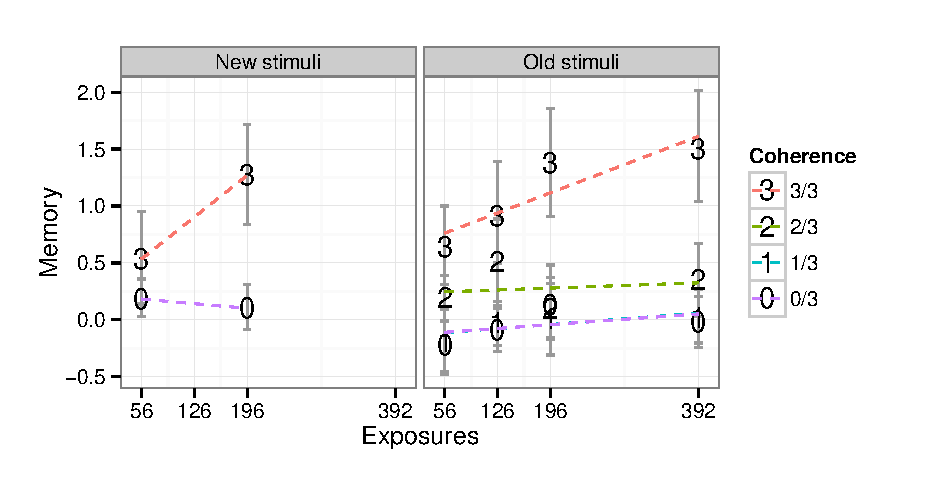
\includegraphics[width=0.7\linewidth]{stim-comparison-mem} \\

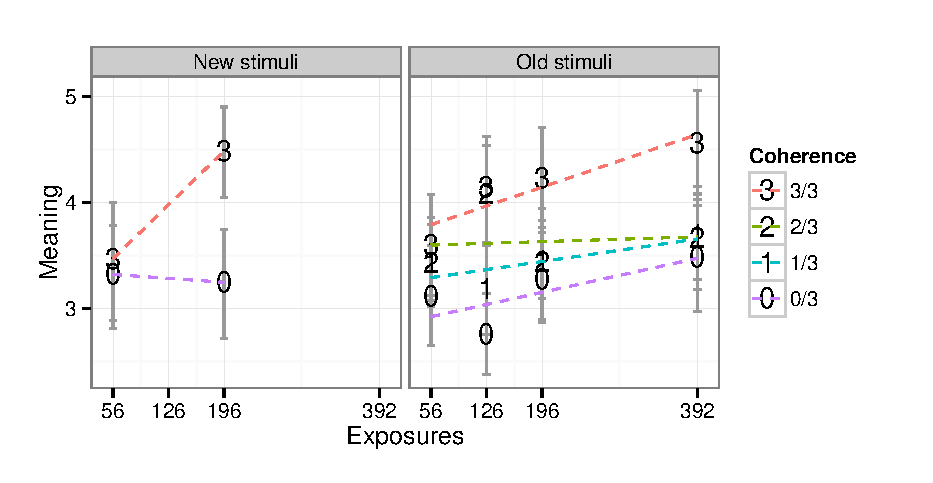
\includegraphics[width=0.7\linewidth]{stim-comparison-mng} \\

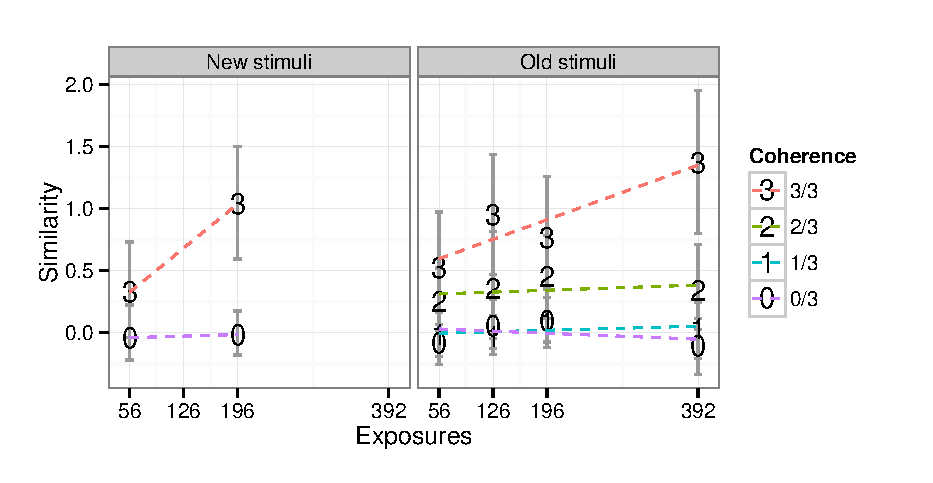
\includegraphics[width=0.7\linewidth]{stim-comparison-sim}
\end{center}


\end{document}

